\section{Joint Segmentation and Tracking}

\begin{frame}{Motivation}
    \begin{figure}
        \centering
        \begin{subfigure}[t]{0.48\textwidth}
            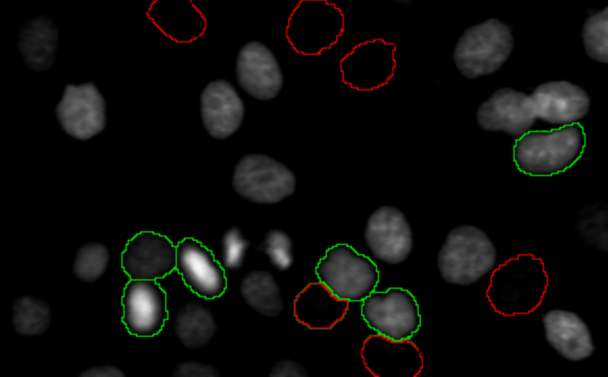
\includegraphics[width=\textwidth]{images/joint/mitocheck_255_max.pdf}
            \caption{Missed cells}
            \label{fig:joint-underseg-no-detection}
        \end{subfigure}
        \hfill
        \begin{subfigure}[t]{0.48\textwidth}
            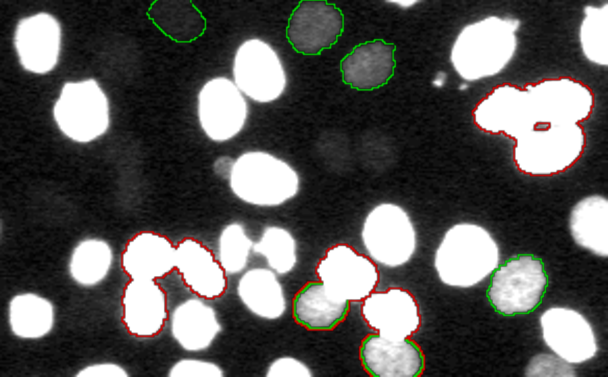
\includegraphics[width=\textwidth]{images/joint/mitocheck_030_max.pdf}
            \caption{Merged objects}
            \label{fig:joint-underseg-mergers}
        \end{subfigure}
    \end{figure}

\end{frame}

\begin{frame}
    \frametitle{Workflow}
    \begin{figure}
        \centering
        \scalebox{0.65}{
            \begin{tikzpicture}
    \newcommand{\distancebetween}{20}
    \newcommand{\shiftdistance}{100}
    \newcommand{\scalingfactor}{0.12}
    \newcommand{\halfscalingfactor}{\scalingfactor}
    
    \begin{scope}
        \begin{scope}[baseline=(raw2)]
    \begin{scope}[yshift=\distancebetween,
        every node/.append style={yslant=0.5,xslant=-1},
        yslant=0.5,xslant=-1]
        \node[inner sep=0, label={[xshift=5]above:{}}] (raw1) {
            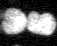
\includegraphics[width=\scalingfactor\textwidth]{images/joint/78_raw_crop_enhanced.png}
        };
    \end{scope}
    \begin{scope}[every node/.append style={yslant=0.5,xslant=-1},yslant=0.5,xslant=-1]
        \begin{pgfonlayer}{bglower}
            \node[inner sep=0, label={[xshift=15]above:{}}] (raw2) {
                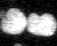
\includegraphics[width=\scalingfactor\textwidth]{images/joint/79_raw_crop_enhanced.png}
            };
        \end{pgfonlayer}
    \end{scope}
    \coordinate (base1) at (raw2.north west |- raw2.south west);
    \coordinate (base2) at (raw2.south east |- raw2.south west);
    % \draw [pllbl]
    % (base1) -- (base2) node[black,midway,yshift=-0.6cm]
    % {Raw Data};
    \path let \p1 = (base1.west), \p2 = (base2.east) in
    node[pllbltxt, minimum width=\x2-\x1] (labelraw) at ($(base1)!0.5!(base2)$)
    {\phantom{g}Raw Data\phantom{g}};
    \begin{pgfonlayer}{bglower}
        \path[threed] (raw2.south east) -- (raw1.south east);
        \path[threed] (raw2.north east) -- (raw1.north east);
        \path[threed] (raw2.south west) -- (raw1.south west);
        \path[threed] (raw2.north west) -- (raw1.north west);
    \end{pgfonlayer}
\end{scope}

%%% Local Variables: 
%%% mode: latex
%%% TeX-master: "../../../main"
%%% End: 

        % \node[ultra thick, left=of raw1,yshift=5mm] {$t\phantom{+1}$};
        % \node[ultra thick, left=of raw2,yshift=5mm] {$t+1$};
        \begin{scope}[xshift=\shiftdistance, baseline=(seg2)]
    \begin{scope}[yshift=\distancebetween,
        every node/.append style={yslant=0.5,xslant=-1},
        yslant=0.5,xslant=-1]
        \node[inner sep=0, label={[xshift=5]above:{}}] (seg1) {
            
\includegraphics[width=\scalingfactor\textwidth]{images/joint/78_seg_crop.png}
        };
    \end{scope}
    \begin{scope}[every node/.append style={yslant=0.5,xslant=-1},yslant=0.5,xslant=-1]
        \begin{pgfonlayer}{bglower}
            \node[inner sep=0, label={[xshift=15]above:{}}] (seg2) {
                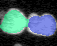
\includegraphics[width=\scalingfactor\textwidth]{images/joint/79_seg_crop.png}
            };
        \end{pgfonlayer}
    \end{scope}
    \coordinate (base1) at (seg2.north west |- seg2.south west);
    \coordinate (base2) at (seg2.south east |- seg2.south west);
    % \draw [pllbl]
    % (base1) -- (base2) node[black,midway,yshift=-0.6cm]
    % {Initial Oversegmentation};
    \path let \p1 = (base1.west), \p2 = (base2.east) in
    node[pllbltxt, minimum width=\x2-\x1] (labelseg) at ($(base1)!0.5!(base2)$) {Oversegmentation};
    \begin{pgfonlayer}{bglower}
        \path[threed] (seg2.south east) -- (seg1.south east);
        \path[threed] (seg2.north east) -- (seg1.north east);
        \path[threed] (seg2.south west) -- (seg1.south west);
        \path[threed] (seg2.north west) -- (seg1.north west);
    \end{pgfonlayer}
\end{scope}

%%% Local Variables: 
%%% mode: latex
%%% TeX-master: "../../../main"
%%% End: 

        \begin{scope}[xshift=2*\shiftdistance, baseline=(cc2)]
    \begin{scope}[yshift=\distancebetween,
        every node/.append style={yslant=0.5,xslant=-1},
        yslant=0.5,xslant=-1]
        \node[inner sep=0, label={[xshift=5]above:{}}] (merge1) {
            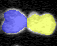
\includegraphics[width=\halfscalingfactor\textwidth]{images/joint/78_merge_crop.png}
        };
        \node[inner sep=0,xshift=47,yshift=-47, label={[xshift=5]above:{}}] (cc1) {
            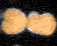
\includegraphics[width=\halfscalingfactor\textwidth]{images/joint/78_cc_crop.png}
        };
    \end{scope}
    \begin{scope}[every node/.append style={yslant=0.5,xslant=-1},yslant=0.5,xslant=-1]
        \begin{pgfonlayer}{bglower}
            \node[inner sep=0, label={[xshift=15]above:{}},rectangle,thin,draw] (merge2) {
                \phantom{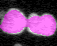
\includegraphics[width=\scalingfactor\textwidth]{images/joint/79_cc_crop.png}}
            };
            \node[xshift=47,yshift=-47,inner sep=0, label={[xshift=15]above:{}}] (cc2) {
                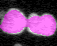
\includegraphics[width=\scalingfactor\textwidth]{images/joint/79_cc_crop.png}
            };
        \end{pgfonlayer}
    \end{scope}
    \coordinate (base1) at (merge1.north west |- cc2.south west);
    \coordinate (base2) at (cc1.south east |- cc2.south west);
    % \draw [pllbl]
    % (base1) -- (base2) node[black,midway,yshift=-0.6cm]
    % {Region Merging};
    \path let \p1 = (base1.west), \p2 = (base2.east) in
    node[pllbltxt, minimum width=\x2-\x1] (labelmerging) at ($(base1)!0.5!(base2)$) {Region Merging};
    \begin{pgfonlayer}{bglower}
        \path[threed] (merge2.south east) -- (merge1.south east);
        \path[threed] (merge2.north east) -- (merge1.north east);
        \path[threed] (merge2.south west) -- (merge1.south west);
        \path[threed] (merge2.north west) -- (merge1.north west);

        \path[threed] (cc2.south east) -- (cc1.south east);
        \path[threed] (cc2.north east) -- (cc1.north east);
        \path[threed] (cc2.south west) -- (cc1.south west);
        \path[threed] (cc2.north west) -- (cc1.north west);
    \end{pgfonlayer}
\end{scope}

%%% Local Variables: 
%%% mode: latex
%%% TeX-master: "../../../main"
%%% End: 

        \begin{pgfonlayer}{background}
            \node[plbg, fit=(raw2.south west) (raw2.north west)
            (raw1.north east) (cc1.south east) (labelraw)] (bg1) {};
        \end{pgfonlayer}
        \draw[arrows=->, ultra thick, transform canvas={xshift=-15}] (bg1.north west) -- (bg1.south
        west) node[midway, xshift=-7] (t1) {\large{$t$}};
    \end{scope}
    \begin{scope}[yshift=-7.5*\distancebetween, xshift=100]
        \begin{scope}
    \begin{scope}[yshift=1.5*\distancebetween,
        every node/.append style={yslant=0.5,xslant=-1},
        yslant=0.5,xslant=-1]
        \node[inner sep=0] (image1) {
            \phantom{
\includegraphics[width=\scalingfactor\textwidth]{images/joint/78_seg_crop.png}}
        };
        \begin{pgfonlayer}{upper}
            \begin{scope}[every node/.append style={scale=0.7}]
                \node[fg_det, label={[font=\tiny]center:$X_1^t$}] (a1) at (image1.south east) {};
                \node[fg_det, label={[font=\tiny]center:$X_2^t$}] (a2) at ($(image1.south east)!0.5!(image1.north east)$) {};
                \node[fg_det, label={[font=\tiny]center:$X_3^t$}] (a3) at (image1.north east) {};
                \node[fg_det, label={[font=\tiny]center:$X_5^t$}] (a5) at ($(image1.south west)!0.5!(image1.north west)$) {};
                \node[fg_det, label={[font=\tiny]center:$X_4^t$}] (a4) at ($(a3)!0.5!(a5)$) {};
            \end{scope}
            \begin{scope}[every node/.append style={scale=0.5}]
                \node[conflict,yshift=-5] (c1) at ($(a1)!0.5!(a5)$) {};
                \node[conflict, right=of a3, xshift=-20, yshift=20] (c2) {};
                \node[conflict, yshift=-20] (c3) at (a4) {};
                \node[count, yshift=-20] (c4)  at ($(a2)!0.5!(a4)$) {};
                
                \path[count] (a1) edge (c4);
                \path[count] (a2) edge (c4);
                \path[count] (a3.south) edge (c4);
                \path[count] (a4) edge (c4);
                \path[count] (a5) edge[bend right=20] (c4);
                
                \path[conflict] (a5) edge[bend right=10] (c1);
                \path[conflict] (a1) edge (c1);

                \path[conflict] (a2) edge (c2);
                \path[conflict] (a4) edge[bend left=100] (c2);
                \path[conflict] (a5) edge[bend left=95] coordinate[pos=0.65](helpercoord1) (c2);

                \path[conflict] (a3) edge[bend left=10] (c3);
                \path[conflict] (a4) edge (c3);
                \path[conflict] (a5) edge (c3);
            \end{scope}
        \end{pgfonlayer}
        \begin{pgfonlayer}{bgupper}
            \node[rectangle, color=black,thick, fill=hypothesesbackground!30, opacity=0.8, draw=black,
            fit=(a1) (c2) (a5) (helpercoord1), inner sep=2, opacity=0.8, label={[xshift=5]above:{}}]
            (bgup) {};
        \end{pgfonlayer}
    \end{scope}
    \begin{scope}[every node/.append style={yslant=0.5,xslant=-1},yslant=0.5,xslant=-1]
        \node[inner sep=0] (image2) {
            \phantom{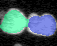
\includegraphics[width=\scalingfactor\textwidth]{images/joint/79_seg_crop.png}}
        };
        \begin{pgfonlayer}{bglower}
            \node[rectangle, color=black,thick, fill=hypothesesbackground!30, opacity=0.8, draw=black,
            fit=(a1) (c2) (a5) (helpercoord1), inner sep=2, opacity=0.8, shift=($(image2) - (image1)$), label={[xshift=15]above:{}}]
            (bglow) {};
        \end{pgfonlayer}
        \begin{pgfonlayer}{lower}
            \begin{scope}[every node/.append style={scale=0.7}]
                \node[fg_det, label={[font=\tiny]center:$X_6^{t+1}$}] (b1) at (image2.south east) {};
                \node[fg_det, label={[font=\tiny]center:$X_7^{t+1}$}] (b2) at (image2.north east) {};
                \node[fg_det, label={[font=\tiny]center:$X_8^{t+1}$}] (b3) at ($(image2.south west)!0.5!(image2.north west)$) {};
            \end{scope}
            \begin{scope}[every node/.append style={scale=0.5}]
                \path[conflict] (b1) edge (b3);
                \path[conflict] (b3) edge (b2);
                \node[conflict] (c1) at ($(b1)!0.5!(b3)$) {};
                \node[conflict] (c2) at ($(b2)!0.5!(b3)$) {};
                \node[count] (c3) at ($(b1)!0.5!(b2)!0.3!(b3)$) {};
                \path[count] (b1) edge (c3);
                \path[count] (b2) edge (c3);
                \path[count] (b3) edge (c3);
            \end{scope}
        \end{pgfonlayer}
    \end{scope}
    \begin{pgfonlayer}{transition}
        \begin{scope}[every node/.append style={scale=0.6}]
            \node[fg_tra,label={[font=\tiny]center:$Y_{1,6}^t$},xshift=30] (trans1) at ($(a1)!0.55!(b1)$) {};
        \end{scope}
        \begin{scope}[every node/.append style={scale=0.2}]
            \node[transfac] (out) at ($(a1.center)!0.5!(trans1)$) {};
            \node[transfac] (in) at ($(b1.center)!0.5!(trans1)$) {};
            \path[transfac] (a1) edge (out.center);
            \path[transfac] (out) edge (trans1);
            \path[transfac] (trans1) edge (in);
            \path[transfac] (in) edge (b1.center);
        \end{scope}
    \end{pgfonlayer}
    \coordinate (base1) at (bglow.north west |- bglow.south west);
    \coordinate (base2) at (bglow.south east |- bglow.south west);
    % \draw [pllbl] (base1) -- (base2) node[black,midway,yshift=-0.6cm] {Factor Graph};
    \path let \p1 = (base1.west), \p2 = (base2.east) in
    node[pllbltxt, minimum width=\x2-\x1] (labelgraph) at ($(base1)!0.5!(base2)$) {Factor Graph};
    \begin{pgfonlayer}{bglower}
        \path[threed] (bglow.south east) -- (bgup.south east);
        \path[threed] (bglow.north east) -- (bgup.north east);
        \path[threed] (bglow.south west) -- (bgup.south west);
        \path[threed] (bglow.north west) -- (bgup.north west);
    \end{pgfonlayer}
\end{scope}

%%% Local Variables: 
%%% mode: latex
%%% TeX-master: "../../../main"
%%% End: 

        % \node[ultra thick, left=of raw1,yshift=5mm] {$t\phantom{+1}$};
        % \node[ultra thick, left=of raw2,yshift=5mm] {$t+1$};
        \begin{scope}[xshift=1.3*\shiftdistance]
    \begin{scope}[yshift=\distancebetween,
        every node/.append style={yslant=0.5,xslant=-1},
        yslant=0.5,xslant=-1]
        \node[inner sep=0, label={[xshift=5]above:{}}] (res1) {
            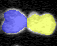
\includegraphics[width=\scalingfactor\textwidth]{images/joint/78_res_crop.png}
        };
    \end{scope}
    \begin{scope}[every node/.append style={yslant=0.5,xslant=-1},yslant=0.5,xslant=-1]
        \begin{pgfonlayer}{bglower}
            \node[inner sep=0, label={[xshift=15]above:{}}] (res2) {
                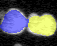
\includegraphics[width=\scalingfactor\textwidth]{images/joint/79_res_crop.png}
            };
        \end{pgfonlayer}
    \end{scope}
    \coordinate (base1) at (res2.north west |- bglow.south west);
    \coordinate (base2) at (res2.south east |- bglow.south west);
    % \draw (base1) rectangle[pllbltxt, yshift=-10] (base2);%  {Tracking Result};
    \path let \p1 = (base1.west), \p2 = (base2.east) in
    node[pllbltxt, minimum width=\x2-\x1]  (labelres) at ($(base1)!0.5!(base2)$) {Tracking Result};
    \begin{pgfonlayer}{bglower}
        \path[threed] (res2.south east) -- (res1.south east);
        \path[threed] (res2.north east) -- (res1.north east);
        \path[threed] (res2.south west) -- (res1.south west);
        \path[threed] (res2.north west) -- (res1.north west);
    \end{pgfonlayer}
\end{scope}

%%% Local Variables: 
%%% mode: latex
%%% TeX-master: "../../../main"
%%% End: 

        \begin{pgfonlayer}{background}
            \node[plbg, fit=(bglow.south west) (bglow.north west)
            (bgup.north east) (res1.south east) (labelres.south)] (bg2) {};
        \end{pgfonlayer}
        \draw[arrows=->, ultra thick, transform canvas={xshift=-15}] (bg2.north west) -- (bg2.south
        west) node[midway, xshift=-7] (t2) {\large{$t$}};
    \end{scope}

    \begin{pgfonlayer}{background}
        \coordinate[xshift=0mm,left=of t1] (hawaii);
        \coordinate[right=of bg1.east,xshift=0mm] (coordeast);
        % \coordinate[below right=of bg1.south east,yshift=-5mm] (coordsouth);
        \coordinate (helper) at ($(bg1.south)!0.5!(bg2.north)$);
        \coordinate (coordsoutheast) at (coordeast |- helper);
        \coordinate[left=of t2.west,xshift=0mm] (coordwestwest);
        \coordinate[xshift=15mm] (coordwest) at (coordwestwest);
        \coordinate (coordsouthwest) at (coordwestwest |- helper);
        \path[arrows=->,draw, line width=4mm, color=red!40, rounded corners=5pt] (hawaii) -- (bg1.east) -- (coordeast) --
(coordsoutheast) -- (coordsouthwest) -- (coordwestwest) -- (coordwest) -- (coordeast |- bg2.east);
    \end{pgfonlayer}
    
\end{tikzpicture}

%%% Local Variables: 
%%% mode: latex
%%% TeX-master: "../../../main"
%%% End: 

        }
        \caption{Joint segmentation and tracking workflow.}
        \label{fig:joint-pipeline}
    \end{figure}
\end{frame}

% \begin{frame}
%     \frametitle{Definitions}
%     \begin{itemize}
%           \item \emph{Segment} or \emph{superpixel/-voxel}: Smallest unit in a segmentation
%           \item \emph{Region}: Any single segment or union of two neighboring regions
%           \item \emph{Conflict}: Set of overlapping and thus contradicting regions
%           \item \emph{Connected Component}: A region that has no neighbors (is completely surrounded
%         by background)
%     \end{itemize}
% \end{frame}

\begin{frame}
    \frametitle{Definitions - Example}
    \begin{minipage}[t][0.4\textheight][t]{\textwidth}%
        \begin{figure}%
            \centering%
            \begin{subfigure}[t]{0.23\textwidth}%
                \centering%
                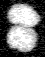
\includegraphics[width=\textwidth]{images/joint/overseg/75/02/raw_contrast.png}
            \end{subfigure}%
            \hfill
            \begin{subfigure}[t]{0.23\textwidth}
                \centering
                \begin{tikzpicture}[baseline=(image1.south)]
                    {\uncover<2->{\node[anchor=south west,inner sep=0] (image1) {
                                
\includegraphics[width=\textwidth]{images/joint/overseg/75/02/colored00.png}};
                            \begin{scope}[x={(image1.south east)},y={(image1.north west)}]
                                \node[region_id] at (0.4, 0.75) {\huge{$3$}};
                                \node[region_id] at (0.65, 0.7) {\huge{$2$}};
                                \node[region_id] at (0.5, 0.32) {\huge{$1$}};
                            \end{scope}}}%
                \end{tikzpicture}%
            \end{subfigure}%
            \hfill%
            \begin{subfigure}[t]{0.23\textwidth}
                \centering
                \begin{tikzpicture}[baseline=(image2.south)]
                    {\uncover<3->{\node[anchor=south west,inner sep=0] (image2) {
                                
\includegraphics[width=\textwidth]{images/joint/overseg/75/02/colored01_all.png}};
                            \begin{scope}[x={(image1.south east)},y={(image2.north west)}]
                                \node[region_id] at (0.53, 0.73) {\huge{$4$}};
                                \node[region_id] at (0.5, 0.32) {\huge{$1$}};
                            \end{scope}}}
                \end{tikzpicture}%
            \end{subfigure}%
            \hfill%
            \begin{subfigure}[t]{0.23\textwidth}
                \centering
                \begin{tikzpicture}[baseline=(image3.south)]
                    {\uncover<4->{\node[anchor=south west,inner sep=0] (image3) {
                                
\includegraphics[width=\textwidth]{images/joint/overseg/75/02/colored02.png}};
                            \begin{scope}[x={(image1.south east)},y={(image3.north west)}]
                                \node[region_id] at (0.5, 0.32) {\huge{$5$}};
                            \end{scope}}}
                \end{tikzpicture}%
            \end{subfigure}%
            \label{fig:joint-segments-example}
        \end{figure}%
    \end{minipage}%
    \begin{overprint}%
        %\only<1-4>{
        \begin{itemize}%
              \item<2-4|only@2-4> Segments: $\{1,2,3\}$%
              \item<2|only@2> Regions: $\{1,2,3\}$%
              \item<3|only@3> Regions: $\{1,2,3,4\}$%
              \item<4|only@4> Regions: $\{1,2,3,4,5\}$%
              \item<4> Connected Component: $\{5\}$%
            %   \item<3|only@3> Conflicts: $\{1,4\},\{2,4\}$%
              \item<4> Conflicts: $\{2,4,5\},\{3,4,5\},\{1,5\}$%
        \end{itemize}%}%
        % \vspace{-50pt}
        \visible<5-|only@5->{
            \begin{figure}
                \centering
                \begin{subfigure}[b]{0.40\textwidth}
                    \begin{flushleft}
                    \scalebox{0.950}{
                    \begin{tikzpicture}[baseline=(bl)]
                        \node[conflict_graph] (r5) {$5$};
                        \node[conflict_graph, right=of r5] (r1) {$3$};
                        \node[conflict_graph, below=of r5] (r2) {$2$};
                        \node[conflict_graph, right=of r2] (r4) {$4$};
                        \node[conflict_graph, left=of r2] (r3) {$1$};
                        \path[conflict_edge] (r5) edge (r1);
                        \path[conflict_edge] (r5) edge (r2);
                        \path[conflict_edge] (r5) edge (r3);
                        \path[conflict_edge] (r5) edge (r4);
                        \path[conflict_edge] (r4) edge (r1);
                        \path[conflict_edge] (r4) edge (r2);
                        \coordinate[below=of r1.south] (bl);
                    \end{tikzpicture}}
                    \end{flushleft}
                \end{subfigure}%
                %\hfill%
                \visible<6-|only@6->{
                    \scalebox{0.7}{
                    \tikzfancyarrow{Factor Graph}}%
                %\hfill%
                \begin{subfigure}[b]{0.40\textwidth}
                    \centering
                    \begin{flushright}
                    \scalebox{0.950}{
                    \begin{tikzpicture}[baseline=(bl)]
                        \node[conflict_graph] (r5) {$5$};
                        \node[conflict_graph, right=of r5] (r1) {$3$};
                        \node[conflict_graph, below=of r5] (r2) {$2$};
                        \node[conflict_graph, right=of r2] (r4) {$4$};
                        \node[conflict_graph, left=of r2] (r3) {$1$};
                        \node[conflict] (c15) at ($(r3)!0.5!(r5)$) {};
                        \node[conflict, xshift=9, yshift=9] (c245) at (r2.north east) {};
                        \node[conflict, xshift=-9, yshift=-9] (c345) at (r1.south west) {};
                        \path[conflict_edge] (r5) edge (c15);
                        \path[conflict_edge] (r3) edge (c15);
                        \path[conflict_edge] (r5) edge (c245);
                        \path[conflict_edge] (r4) edge (c245);
                        \path[conflict_edge] (r2) edge (c245);
                        \path[conflict_edge] (r5) edge (c345);
                        \path[conflict_edge] (r4) edge (c345);
                        \path[conflict_edge] (r1) edge (c345);
                        \coordinate[below=of r1.south] (bl);
                    \end{tikzpicture}}
                \end{flushright}%
                \end{subfigure}}%
            \end{figure}
        }%
    \end{overprint}%
\end{frame}


\begin{frame}
    \frametitle{From Regions to Factor Graph}
    \begin{minipage}[t][0.4\textheight][t]{\textwidth}%
        \begin{figure}
            \centering
            \begin{subfigure}[t]{0.23\textwidth}
                \centering
                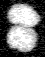
\includegraphics[width=\textwidth]{images/joint/overseg/75/02/raw_contrast.png}
                % \caption{Raw data}
            \end{subfigure}%
            \hfill%
            \begin{subfigure}[t]{0.23\textwidth}
                \centering
                \begin{tikzpicture}[baseline=(image1.south)]
                    \node[anchor=south west,inner sep=0] (image1) {
                        
\includegraphics[width=\textwidth]{images/joint/overseg/75/02/colored00.png}};
                    \begin{scope}[x={(image1.south east)},y={(image1.north west)}]
                        \node[region_id] at (0.4, 0.75) {\huge{$3$}};
                        \node[region_id] at (0.65, 0.7) {\huge{$2$}};
                        \node[region_id] at (0.5, 0.32) {\huge{$1$}};
                    \end{scope}
                \end{tikzpicture}%
            \end{subfigure}%
            \hfill%
            \begin{subfigure}[t]{0.23\textwidth}
                \centering
                \begin{tikzpicture}[baseline=(image2.south)]
                    \node[anchor=south west,inner sep=0] (image2) {
                        
\includegraphics[width=\textwidth]{images/joint/overseg/75/02/colored01_all.png}};
                    \begin{scope}[x={(image1.south east)},y={(image2.north west)}]
                        \node[region_id] at (0.53, 0.73) {\huge{$4$}};
                        \node[region_id] at (0.5, 0.32) {\huge{$1$}};
                    \end{scope}
                \end{tikzpicture}%
            \end{subfigure}%
            \hfill%
            \begin{subfigure}[t]{0.23\textwidth}
                \centering
                \begin{tikzpicture}[baseline=(image3.south)]
                    \node[anchor=south west,inner sep=0] (image3) {
                        
\includegraphics[width=\textwidth]{images/joint/overseg/75/02/colored02.png}};
                    \begin{scope}[x={(image1.south east)},y={(image3.north west)}]
                        \node[region_id] at (0.5, 0.32) {\huge{$5$}};
                    \end{scope}
                \end{tikzpicture}%
            \end{subfigure}%
        \end{figure}
    \end{minipage}%
    % 
    \begin{figure}
        \centering
        \newcommand{\scalingfactor}{0.3}
        \scalebox{0.9}{
            \begin{tikzpicture}
                \begin{scope}
    \begin{scope}[
        every node/.append style={yslant=0.5,xslant=-1},
        yslant=0.5,xslant=-1]
        \node[inner sep=0] (image1) {
            \phantom{
\includegraphics[width=\scalingfactor\textwidth]{images/joint/78_seg_crop.png}}
        };
        \begin{pgfonlayer}{upper}
            \begin{scope}[every node/.append style={scale=0.7}]
                \node[fg_det, label={[font=\tiny]center:$X_1^t$}] (a1) at (image1.south east) {};
                \node[fg_det, label={[font=\tiny]center:$X_2^t$}] (a2) at ($(image1.south east)!0.5!(image1.north east)$) {};
                \node[fg_det, label={[font=\tiny]center:$X_3^t$}] (a3) at (image1.north east) {};
                \node[fg_det, label={[font=\tiny]center:$X_5^t$}] (a5) at ($(image1.south west)!0.5!(image1.north west)$) {};
                \node[fg_det, label={[font=\tiny]center:$X_4^t$}] (a4) at ($(a3)!0.5!(a5)$) {};
            \end{scope}
            \begin{scope}[every node/.append style={scale=0.65}]
                \node[conflict,yshift=-5] (c1) at ($(a1)!0.5!(a5)$) {};
                \node[conflict, right=of a3, xshift=-20, yshift=20] (c2) {};
                \node[conflict, yshift=-20] (c3) at (a4) {};
                \node[count, yshift=-20] (c4)  at ($(a2)!0.5!(a4)$) {};
                
                \path[count] (a1) edge (c4);
                \path[count] (a2) edge (c4);
                \path[count] (a3.south) edge (c4);
                \path[count] (a4) edge (c4);
                \path[count] (a5) edge[bend right=20] (c4);
                
                \path[conflict] (a5) edge[bend right=10] (c1);
                \path[conflict] (a1) edge (c1);

                \path[conflict] (a2) edge (c2);
                \path[conflict] (a4) edge[bend left=100] (c2);
                \path[conflict] (a5) edge[bend left=95] coordinate[pos=0.65](helpercoord1) (c2);

                \path[conflict] (a3) edge[bend left=10] (c3);
                \path[conflict] (a4) edge (c3);
                \path[conflict] (a5) edge (c3);
            \end{scope}
        \end{pgfonlayer}
        \begin{pgfonlayer}{bgupper}
            \node[rectangle, color=black,thick, fill=hypothesesbackground!30, opacity=0.8, draw=black,
            fit=(a1) (c2) (a5) (helpercoord1), inner sep=2, opacity=0.8, label={[xshift=5]above:{}}]
            (bgup) {};
        \end{pgfonlayer}
    \end{scope}
\end{scope}


%%% Local Variables: 
%%% mode: latex
%%% TeX-master: "../../main"
%%% End: 

            \end{tikzpicture}
        }
    \end{figure}
\end{frame}


\begin{frame}
    \frametitle{Graphical Model}
    \centering
    \newcommand{\distancebetweenlayers}{90}
    \newcommand{\scalingfactor}{0.3}
    \scalebox{0.8}{
        \begin{tikzpicture}
            \begin{scope}
    
    \begin{scope}[yshift=\distancebetweenlayers,
        every node/.append style={yslant=-0.5,xslant=1},
        yslant=-0.5,xslant=1]
        \node[inner sep=0] (image1) {
            \phantom{
\includegraphics[width=\scalingfactor\textwidth]{images/joint/78_seg_crop.png}}
        };
        \begin{pgfonlayer}{upper}
            \begin{scope}[every node/.append style={scale=0.7}]
                \node[fg_det, label={[font=\tiny]center:$X_1^t$}] (a1) at (image1.south east) {};
                \node[fg_det, label={[font=\tiny]center:$X_2^t$}] (a2) at ($(image1.south east)!0.5!(image1.north east)$) {};
                \node[fg_det, label={[font=\tiny]center:$X_3^t$}] (a3) at (image1.north east) {};
                \node[fg_det, label={[font=\tiny]center:$X_5^t$}] (a5) at ($(image1.south west)!0.5!(image1.north west)$) {};
                \node[fg_det, label={[font=\tiny]center:$X_4^t$}] (a4) at ($(a3)!0.5!(a5)$) {};
            \end{scope}
            \begin{scope}[every node/.append style={scale=0.65}]
                \node[conflict,yshift=-5] (c1) at ($(a1)!0.5!(a5)$) {};
                \node[conflict, right=of a3, xshift=-10, yshift=-10] (c2) {};
                \node[conflict, yshift=-20] (c3) at (a4) {};
                \node[count, yshift=-20] (c4)  at ($(a2)!0.5!(a4)$) {};
                
                \path[count] (a1) edge (c4);
                \path[count] (a2) edge (c4);
                \path[count] (a3.south) edge (c4);
                \path[count] (a4) edge (c4);
                \path[count] (a5) edge[bend right=20] (c4);
                
                \path[conflict] (a5) edge[bend right=10] (c1);
                \path[conflict] (a1) edge (c1);

                \path[conflict] (a2) edge (c2);
                \path[conflict] (a4) edge[bend left=50] (c2);
                \path[conflict] (a5) edge[bend left=65] coordinate[pos=0.65](helpercoord1) (c2);

                \path[conflict] (a3) edge[bend left=10] (c3);
                \path[conflict] (a4) edge (c3);
                \path[conflict] (a5) edge (c3);
            \end{scope}
        \end{pgfonlayer}
        \begin{pgfonlayer}{bgupper}
            \node[rectangle, color=black,thick, fill=hypothesesbackground!30, opacity=0.8, draw=black,
            fit=(a1) (c2) (a5) (helpercoord1), inner sep=2, opacity=0.8, label={[xshift=15]above:{$t\phantom{+1}$}}]
            (bgup) {};
        \end{pgfonlayer}
    \end{scope}

    \begin{scope}[every node/.append style={yslant=-0.5,xslant=1},yslant=-0.5,xslant=1]
        \node[inner sep=0] (image2) {
            \phantom{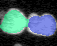
\includegraphics[width=\scalingfactor\textwidth]{images/joint/79_seg_crop.png}}
        };
        
        \begin{pgfonlayer}{bglower}
            \uncover<2->{
            \node[rectangle, color=black,thick, fill=hypothesesbackground!30, opacity=0.8, draw=black,
            fit=(a1) (c2) (a5) (helpercoord1), inner sep=2, opacity=0.8, shift=($(image2) - (image1)$), label={[xshift=15]above:{$t+1$}}]
            (bglow) {};
            }
        \end{pgfonlayer}
        \begin{pgfonlayer}{lower}
            \uncover<2->{
            \begin{scope}[every node/.append style={scale=0.7}]
                \node[fg_det, label={[font=\tiny]center:$X_6^{t+1}$}] (b1) at (image2.south east) {};
                \node[fg_det, label={[font=\tiny]center:$X_7^{t+1}$}] (b2) at (image2.north east) {};
                \node[fg_det, label={[font=\tiny]center:$X_8^{t+1}$}] (b3) at ($(image2.south west)!0.5!(image2.north west)$) {};
            \end{scope}
            \begin{scope}[every node/.append style={scale=0.65}]
                \path[conflict] (b1) edge (b3);
                \path[conflict] (b3) edge (b2);
                \node[conflict, label=below left:$\psi_{\text{det}}$] (c1) at ($(b1)!0.5!(b3)$) {};
                \node[conflict] (c2) at ($(b2)!0.5!(b3)$) {};
                \node[count, label={[yshift=3mm]right:$\psi_{\text{count}}$}] (c3) at ($(b1)!0.5!(b2)!0.3!(b3)$) {};
                \path[count] (b1) edge (c3);
                \path[count] (b2) edge (c3);
                \path[count] (b3) edge (c3);
            \end{scope}
            }
        \end{pgfonlayer}
    \end{scope}

    \begin{pgfonlayer}{transition}
        \uncover<3->{
        \begin{scope}[every node/.append style={scale=0.9}]
            \node[fg_tra,label={[font=\tiny]center:$Y_{1,6}^t$},xshift=0] (trans1) at ($(a1)!0.55!(b1)$) {};
        \end{scope}
        \begin{scope}[every node/.append style={scale=0.7}]
            \node[transfac, label=left:$\psi_{\text{out}}$] (out) at ($(a1.center)!0.5!(trans1)$) {};
            \node[transfac] (in) at ($(b1.center)!0.5!(trans1)$) {};
            \path[transfac] (a1) edge (out.center);
            \path[transfac] (out) edge (trans1);
            \path[transfac] (trans1) edge (in);
            \path[transfac] (in) edge (b1.center);
        \end{scope}
        \begin{scope}[every node/.append style={scale=0.9}]
            \node[fg_tra,label={[font=\tiny]center:$Y_{1,7}^t$},xshift=0,yshift=0] (trans2) at ($(out)!0.35!(b2)$) {};
        \end{scope}
        \begin{scope}[every node/.append style={scale=0.7}]
            \node[transfac, label={[yshift=3mm]right:$\psi_{\text{in}}$}] (in2) at ($(b2.center)!0.5!(trans2)$) {};
            \path[transfac] (out) edge (trans2);
            \path[transfac] (trans2) edge (in2);
            \path[transfac] (in2) edge (b2.center);
        \end{scope}
        }
    \end{pgfonlayer}
    \coordinate (base1) at (bglow.north west |- bglow.south west);
    \coordinate (base2) at (bglow.south east |- bglow.south west);
    % \draw [pllbl] (base1) -- (base2) node[black,midway,yshift=-0.6cm] {Factor Graph};
    % \path let \p1 = (base1.west), \p2 = (base2.east) in
    % node[pllbltxt, minimum width=\x2-\x1] (labelgraph) at ($(base1)!0.5!(base2)$) {Factor Graph};
\end{scope}


%%% Local Variables: 
%%% mode: latex
%%% TeX-master: "../../main"
%%% End: 

        \end{tikzpicture}
    }\hfill%
    \scalebox{0.8}{
        \begin{tikzpicture}%
            \visible<1->{
                \begin{scope}
                    \node[circle, draw, thick] (a11) {$1$};
                    \node[circle, draw, thick, right=of a11, xshift=-15] (a12) {$2$};
                    \node[circle, draw, thick, right=of a12, xshift=-15] (a13) {$3$};
                    \node[circle, draw, thick, above=of a12, yshift=10] (a15) {$5$};
                    \node[circle, draw, thick] (a14) at ($(a15)!0.5!(a13)$) {$4$};
                    \path (a11) edge (a15);
                    \path (a14) edge (a15);
                    \path (a12) edge (a14);
                    \path (a13) edge (a14);
                \end{scope}
            }%
            \visible<2->{
                \begin{scope}[yshift=-120]
                    \node[circle, draw, thick] (a21) {$6$};
                    \node[circle, draw, thick, opacity=0.0, right=of a21, xshift=-15] (fake1) {$6$};
                    \node[circle, draw, thick, right=of fake1, xshift=-15] (a22) {$7$};
                    \node[circle, draw, thick, above=of fake1, yshift=10] (a23) {$8$};
                    \path (a21) edge (a23);
                    \path (a22) edge (a23);
                \end{scope}
            }%
        \end{tikzpicture}}%
    \vfill
    % \caption{Factor Graph}
    \begin{minipage}{0.33\textwidth}
        \begin{tabular}{ll}
            \tikz[baseline, inner sep=1pt]\node[scale=0.4, thick, draw, circle, fg_det, text=black] at
            (0,2.5pt){$X$}; & Detection \\
            \uncover<3->{\tikz[baseline, inner sep=1pt]\node[scale=0.4, thick, draw, circle, fg_tra, text=black] at
                (0,2.5pt){$Y$};} & \uncover<3->{Assignment} \\
        \end{tabular}
    \end{minipage}%
    \begin{minipage}{0.33\textwidth}
        \begin{tabular}{ll}
            \tikz[baseline, inner sep=1pt]{\node[scale=2.5, thick, draw, circle, conflict] (c1) at
                (0,2.8pt){};
                \node[opacity=0.0, fg_det, scale=0.4] (fake) at (c1.center) {\phantom{$X$}};
                \path[conflict] (fake.west) edge (fake.east);
            }
            & Conflict \\
            \uncover<3->{\tikz[baseline, inner sep=1pt]{\node[scale=2.5, thick, draw, rectangle, transfac] (c1) at
                    (0,2.8pt){};
                    \node[opacity=0.0, fg_det, scale=0.4] (fake) at (c1.center) {\phantom{$X$}};
                    \path[transfac] (fake.west) edge (fake.east);
                }
            }
            & \uncover<3->{Outgoing} \\
        \end{tabular}
    \end{minipage}%
    \begin{minipage}{0.33\textwidth}
        \begin{tabular}{ll}
            \tikz[baseline, inner sep=1pt]{\node[scale=2.5, thick, draw, count] (c1) at
                (0,2.8pt){};
                \node[opacity=0.0, fg_det, scale=0.4] (fake) at (c1.center) {\phantom{$X$}};
                \path[count] (fake.west) edge (fake.east);
            }
            & Count \\
            \uncover<3->{\tikz[baseline, inner sep=1pt]{\node[scale=2.5, thick, draw, rectangle, transfac] (c1) at
                    (0,2.8pt){};
                    \node[opacity=0.0, fg_det, scale=0.4] (fake) at (c1.center) {\phantom{$X$}};
                    \path[transfac] (fake.west) edge (fake.east);
                }
            }
            & \uncover<3->{Incoming} \\
        \end{tabular}
    \end{minipage}
\end{frame}

\begin{frame}{Graphical Model - Wrap-Up}
    \newsavebox{\detVar}
    \savebox{\detVar}{\tikz[baseline, inner sep=1pt]\node[scale=0.4, thick, draw, circle, fg_det, text=black] at
        (0,2.5pt){$X$};}
    \newsavebox{\transVar}
    \savebox{\transVar}{\tikz[baseline, inner sep=1pt]\node[scale=0.4, thick, draw, circle, fg_tra, text=black] at
        (0,2.5pt){$Y$};}
    \newsavebox{\detFac}
    \savebox{\detFac}{\tikz[baseline, inner sep=1pt]{\node[scale=2.5, thick, draw, circle, conflict] (c1) at
            (0,2.8pt){};
            \node[opacity=0.0, fg_det, scale=0.4] (fake) at (c1.center) {\phantom{$X$}};
            \path[conflict] (fake.west) edge (fake.east);
        }}
    \newsavebox{\countFac}
    \savebox{\countFac}{\tikz[baseline, inner sep=1pt]{\node[scale=2.5, thick, draw, circle, count] (c1) at
            (0,2.8pt){};
            \node[opacity=0.0, fg_det, scale=0.4] (fake) at (c1.center) {\phantom{$X$}};
            \path[count] (fake.west) edge (fake.east);
        }}
    \newsavebox{\outFac}
    \savebox{\outFac}{\tikz[baseline, inner sep=1pt]{\node[scale=2.5, thick, draw, circle, transfac] (c1) at
            (0,2.8pt){};
            \node[opacity=0.0, fg_det, scale=0.4] (fake) at (c1.center) {\phantom{$X$}};
            \path[transfac] (fake.west) edge (fake.east);
        }}
    \newsavebox{\inFac}
    \savebox{\inFac}{\tikz[baseline, inner sep=1pt]{\node[scale=2.5, thick, draw, circle, transfac] (c1) at
            (0,2.8pt){};
            \node[opacity=0.0, fg_det, scale=0.4] (fake) at (c1.center) {\phantom{$X$}};
            \path[transfac] (fake.west) edge (fake.east);
        }}
    \begin{minipage}{0.71\textwidth}
        \begin{itemize}
              \item Random Variables
            \begin{itemize}
                  \item[\usebox{\detVar}] Detection
                  \item[\usebox{\transVar}] Assignment
            \end{itemize}
              \item Factors
            \begin{itemize}
                  \item[\usebox{\detFac}] Conflict or Detection factor $\psi_{\text{det}}$
                \begin{itemize}
                      \item[] Detection priors
                      \item[] Conflict constraints
                \end{itemize}
                  \item[\usebox{\countFac}] Count Factor $\psi_{\text{count}}$
                \begin{itemize}
                      \item[] Count prior
                \end{itemize}
                  \item[\usebox{\outFac}] Outgoing Factor $\psi_{\text{out}}$
                \begin{itemize}
                      \item[] Move and Division priors
                      \item[] Assignment Consistency Constraints
                \end{itemize}
                  \item[\usebox{\inFac}] Incoming Factor $\psi_{\text{in}}$
                \begin{itemize}
                      \item[] Assignment Consistency Constraints
                \end{itemize}
            \end{itemize}
        \end{itemize}
    \end{minipage}
    \begin{minipage}{0.25\textwidth}
        \newcommand{\distancebetweenlayers}{60}
        \newcommand{\scalingfactor}{0.8}
        \scalebox{0.55}{
            \begin{tikzpicture}[every node/.append style={scale=0.98}]
                \begin{scope}
    
    \begin{scope}[yshift=\distancebetweenlayers,
        every node/.append style={yslant=0.5,xslant=-1},
        yslant=0.5,xslant=-1]
        \node[inner sep=0] (image1) {
            \phantom{
\includegraphics[width=\scalingfactor\textwidth]{images/joint/78_seg_crop.png}}
        };
        \begin{pgfonlayer}{upper}
            \begin{scope}[every node/.append style={scale=0.7}]
                \node[fg_det, label={[font=\tiny]center:$X_1^t$}] (a1) at (image1.south east) {};
                \node[fg_det, label={[font=\tiny]center:$X_2^t$}] (a2) at ($(image1.south east)!0.5!(image1.north east)$) {};
                \node[fg_det, label={[font=\tiny]center:$X_3^t$}] (a3) at (image1.north east) {};
                \node[fg_det, label={[font=\tiny]center:$X_5^t$}] (a5) at ($(image1.south west)!0.5!(image1.north west)$) {};
                \node[fg_det, label={[font=\tiny]center:$X_4^t$}] (a4) at ($(a3)!0.5!(a5)$) {};
            \end{scope}
            \begin{scope}[every node/.append style={scale=0.65}]
                \node[conflict,yshift=-5] (c1) at ($(a1)!0.5!(a5)$) {};
                \node[conflict, right=of a3, xshift=-20, yshift=20] (c2) {};
                \node[conflict, yshift=-20] (c3) at (a4) {};
                \node[count, yshift=-20] (c4)  at ($(a2)!0.5!(a4)$) {};
                
                \path[count] (a1) edge (c4);
                \path[count] (a2) edge (c4);
                \path[count] (a3.south) edge (c4);
                \path[count] (a4) edge (c4);
                \path[count] (a5) edge[bend right=20] (c4);
                
                \path[conflict] (a5) edge[bend right=10] (c1);
                \path[conflict] (a1) edge (c1);

                \path[conflict] (a2) edge (c2);
                \path[conflict] (a4) edge[bend left=100] (c2);
                \path[conflict] (a5) edge[bend left=95] coordinate[pos=0.65](helpercoord1) (c2);

                \path[conflict] (a3) edge[bend left=10] (c3);
                \path[conflict] (a4) edge (c3);
                \path[conflict] (a5) edge (c3);
            \end{scope}
        \end{pgfonlayer}
        \begin{pgfonlayer}{bgupper}
            \node[rectangle, color=black,thick, fill=hypothesesbackground!30, opacity=0.8, draw=black,
            fit=(a1) (c2) (a5) (helpercoord1), inner sep=2, opacity=0.8, label={[xshift=15]above:{$t\phantom{+1}$}}]
            (bgup) {};
        \end{pgfonlayer}
    \end{scope}

    \begin{scope}[every node/.append style={yslant=0.5,xslant=-1},yslant=0.5,xslant=-1]
        \node[inner sep=0] (image2) {
            \phantom{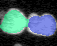
\includegraphics[width=\scalingfactor\textwidth]{images/joint/79_seg_crop.png}}
        };
        
        \begin{pgfonlayer}{bglower}
            \node[rectangle, color=black,thick, fill=hypothesesbackground!30, opacity=0.8, draw=black,
            fit=(a1) (c2) (a5) (helpercoord1), inner sep=2, opacity=0.8, shift=($(image2) - (image1)$), label={[xshift=15]above:{$t+1$}}]
            (bglow) {};
        \end{pgfonlayer}
        \begin{pgfonlayer}{lower}
            \begin{scope}[every node/.append style={scale=0.7}]
                \node[fg_det, label={[font=\tiny]center:$X_6^{t+1}$}] (b1) at (image2.south east) {};
                \node[fg_det, label={[font=\tiny]center:$X_7^{t+1}$}] (b2) at (image2.north east) {};
                \node[fg_det, label={[font=\tiny]center:$X_8^{t+1}$}] (b3) at ($(image2.south west)!0.5!(image2.north west)$) {};
            \end{scope}
            \begin{scope}[every node/.append style={scale=0.65}]
                \path[conflict] (b1) edge (b3);
                \path[conflict] (b3) edge (b2);
                \node[conflict, label=below left:$\psi_{\text{det}}$] (c1) at ($(b1)!0.5!(b3)$) {};
                \node[conflict] (c2) at ($(b2)!0.5!(b3)$) {};
                \node[count, label=right:$\psi_{\text{count}}$] (c3) at ($(b1)!0.5!(b2)!0.3!(b3)$) {};
                \path[count] (b1) edge (c3);
                \path[count] (b2) edge (c3);
                \path[count] (b3) edge (c3);
            \end{scope}
        \end{pgfonlayer}
    \end{scope}

    \begin{pgfonlayer}{transition}
        \begin{scope}[every node/.append style={scale=0.9}]
            \node[fg_tra,label={[font=\tiny]center:$Y_{1,6}^t$},xshift=0] (trans1) at ($(a1)!0.55!(b1)$) {};
        \end{scope}
        \begin{scope}[every node/.append style={scale=0.7}]
            \node[transfac, label=right:$\psi_{\text{out}}$] (out) at ($(a1.center)!0.5!(trans1)$) {};
            \node[transfac, label=right:$\psi_{\text{in}}$] (in) at ($(b1.center)!0.5!(trans1)$) {};
            \path[transfac] (a1) edge (out.center);
            \path[transfac] (out) edge (trans1);
            \path[transfac] (trans1) edge (in);
            \path[transfac] (in) edge (b1.center);
        \end{scope}
        \begin{scope}[every node/.append style={scale=0.9}]
            \node[fg_tra,label={[font=\tiny]center:$Y_{1,7}^t$},xshift=0,yshift=0] (trans2) at ($(out)!0.35!(b2)$) {};
        \end{scope}
        \begin{scope}[every node/.append style={scale=0.7}]
            \node[transfac] (in2) at ($(b2.center)!0.5!(trans2)$) {};
            \path[transfac] (out) edge (trans2);
            \path[transfac] (trans2) edge (in2);
            \path[transfac] (in2) edge (b2.center);
        \end{scope}
    \end{pgfonlayer}
    \coordinate (base1) at (bglow.north west |- bglow.south west);
    \coordinate (base2) at (bglow.south east |- bglow.south west);
    % \draw [pllbl] (base1) -- (base2) node[black,midway,yshift=-0.6cm] {Factor Graph};
    % \path let \p1 = (base1.west), \p2 = (base2.east) in
    % node[pllbltxt, minimum width=\x2-\x1] (labelgraph) at ($(base1)!0.5!(base2)$) {Factor Graph};
\end{scope}


%%% Local Variables: 
%%% mode: latex
%%% TeX-master: "../../main"
%%% End: 

            \end{tikzpicture}
        }\hfill
        \vfill
    \end{minipage}
\end{frame}

\begin{frame}[shrink=25]
    \frametitle{Graphical Model - Joint Probability}
    \begin{align*}
        P(\mathcal{X},\mathcal{Y}) = \frac{1}{Z}\prod_t\prod_i
        \Bigg(&\psi_{\text{count}}(\{X_{i\alpha}^t\}_{\alpha \in I_i^t},f_{i}^t) \\ \nonumber
        &\times\prod_{\alpha}\Big(\psi_{\mathrm{out}}(X_{i\alpha}^t, \mathcal{Y}_{i\alpha\rightarrow}^{t},
        f_{i\alpha}^t, \Xi_{i\alpha\rightarrow}^{t}) \cdot \psi_{\mathrm{in}}(X_{i\alpha}^{t},
        \mathcal{Y}_{\rightarrow i\alpha}^{t-1})\Big) \\ \nonumber
        &\times\prod_{\nu}\Big(\psi_{\text{det}}(\mathcal{K}_{i\nu}^t, \xi_{i\nu}^t)\Big)\Bigg)
    \end{align*}
    \vspace{10pt}
    \begin{center}
        \Large{$\Rightarrow$ Find MAP solution with integer linear programming.}
    \end{center}
\end{frame}

% \begin{frame}
%     \frametitle{Classifiers}
%     Details zu den Classifiern
% \end{frame}

\begin{frame}
    \frametitle{Experiments}
    \begin{figure}
        \centering
        \begin{tikzpicture}
            \node[label=above:{$t=74$}] (seg1) {
\includegraphics[width=0.2\textwidth]{images/joint/res/sequence_01/overseg_raw74.png}};
            \node[label=above:{$t=75$}, right=of seg1.center] (seg2) {
\includegraphics[width=0.2\textwidth]{images/joint/res/sequence_01/overseg_raw75.png}};
            \node[label=above:{$t=76$}, right=of seg2.center] (seg3) {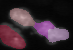
\includegraphics[width=0.2\textwidth]{images/joint/res/sequence_01/overseg_raw76.png}};
            \node[align=center, left=of seg1.center] {Over- \\ segmentation};
            \uncover<2->{
                \node[below=of seg1.center] (tra1) {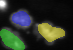
\includegraphics[width=0.2\textwidth]{images/joint/res/sequence_01/ov_raw74.png}};
                \node[below=of seg2.center] (tra2) {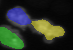
\includegraphics[width=0.2\textwidth]{images/joint/res/sequence_01/ov_raw75.png}};
                \node[below=of seg3.center] (tra3) {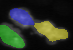
\includegraphics[width=0.2\textwidth]{images/joint/res/sequence_01/ov_raw76.png}};
                \node[align=center, left=of tra1.center] {Tracking};
            }
        \end{tikzpicture}
    \end{figure}
\end{frame}

\begin{frame}
    \frametitle{Experiments}
    \begin{figure}
        \centering
        \begin{tikzpicture}
            \node[label=above:{$t=82$}] (seg1) {
\includegraphics[width=0.2\textwidth]{images/joint/res/sequence_02/overseg_raw82.png}};
            \node[label=above:{$t=83$}, right=of seg1.center] (seg2) {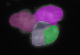
\includegraphics[width=0.2\textwidth]{images/joint/res/sequence_02/overseg_raw83.png}};
            \node[label=above:{$t=84$}, right=of seg2.center] (seg3) {
\includegraphics[width=0.2\textwidth]{images/joint/res/sequence_02/overseg_raw84.png}};
            \node[align=center, left=of seg1.center] {Over- \\ segmentation};
            \uncover<2->{
                \node[below=of seg1.center] (tra1) {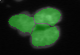
\includegraphics[width=0.2\textwidth]{images/joint/res/sequence_02/ov_raw82.png}};
                \node[below=of seg2.center] (tra2) {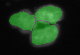
\includegraphics[width=0.2\textwidth]{images/joint/res/sequence_02/ov_raw83.png}};
                \node[below=of seg3.center] (tra3) {
\includegraphics[width=0.2\textwidth]{images/joint/res/sequence_02/ov_raw84.png}};
                \node[align=center, left=of tra1.center] {Tracking};
            }
        \end{tikzpicture}
    \end{figure}
\end{frame}

\begin{frame}[shrink=25]
    \frametitle{Experiments}
    \begin{figure}
        \centering
        \begin{tikzpicture}
            \node[label={[yshift=-2.5mm]above:\small{Segmentation}}] (seg1) {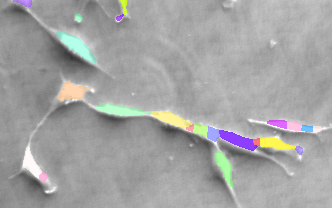
\includegraphics[width=0.32\textwidth]{images/joint/res/sequence_03/00_colored00_raw.png}};
            \node[label={[yshift=-2.5mm]above:\small{Region Merging}}, right=of seg1] (seg2) {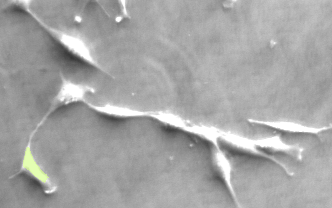
\includegraphics[width=0.32\textwidth]{images/joint/res/sequence_03/00_colored01_raw.png}};
            \node[label={[yshift=-2.5mm]above:\small{Region Merging}}, below=of seg1, yshift=7.5mm] (seg3) {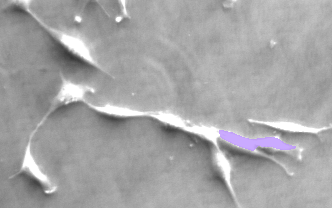
\includegraphics[width=0.32\textwidth]{images/joint/res/sequence_03/00_colored02_raw.png}};
            \node[label={[yshift=-2.5mm]above:\small{Region Merging}}, right=of seg3] (seg4) {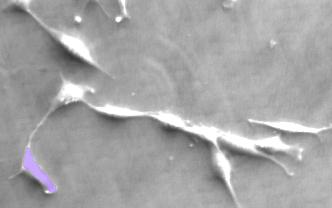
\includegraphics[width=0.32\textwidth]{images/joint/res/sequence_03/00_colored03_raw.png}};
            \node[label={[yshift=-2.5mm]above:\small{Region Merging}}, below=of seg3, yshift=7.5mm] (seg5)  {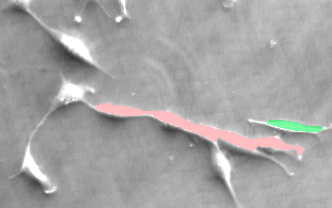
\includegraphics[width=0.32\textwidth]{images/joint/res/sequence_03/00_colored04_raw.png}};
            \node[label={[yshift=-2.5mm]above:\small{Tracking}}, right=of seg5] (tra1) {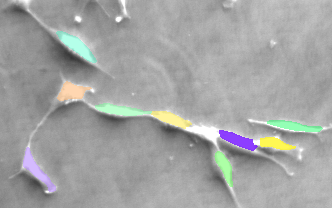
\includegraphics[width=0.32\textwidth]{images/joint/res/sequence_03/00_track_raw.png}};
        \end{tikzpicture}
    \end{figure}
\end{frame}

\begin{frame}
    \frametitle{Open Challenges}
    \renewcommand{\arraystretch}{1.5}
    \begin{tabularx}{\textwidth}{X|X}
        Challenge & Solution \\ \hline
        Region merging errors propagated into tracking result  & Improve region merging (vigra) \\
        Tractability & Change hypotheses generation \\
        Parameters not optimal & Do exhaustive grid search \\
    \end{tabularx}
\end{frame}

\begin{frame}
    \begin{center}
        Thank you!
    \end{center}
\end{frame}


%%% Local Variables: 
%%% mode: latex
%%% TeX-master: "../main"
%%% End: 
